\documentclass[hidelinks,10pt,letter]{article} % KOMA-Script article scrartcl
\usepackage{lipsum}
\usepackage{url}
\usepackage[nochapters]{classicthesis}
\usepackage{authordate1-4}
\usepackage{graphicx}
\usepackage{amsmath}
\usepackage{enumerate}

\begin{document}
    \title{\rmfamily\normalfont\spacedallcaps{Visualizing Machine~Translation~Quality for Monolinguals}}
    \author{\spacedlowsmallcaps{Marianna Rapoport}}
    \date{}
    
    \maketitle
    
    \setcounter{tocdepth}{1}
    
    \newcommand{\dash}{~--- }
    
    \begin{abstract}
        \noindent This article proposes an extension for machine translators
        that aims to help users without knowledge of the target language to
        improve the quality of the translation. The extension highlights subphrases in the 
        source text according to the faithfulness of their translation and fluency
        in the source language. This allows users to assess
        the quality of the translation and eventually improve it by paraphrasing 
        the highlighted expressions.
    \end{abstract}
       
    \tableofcontents
    
    \section{Introduction}\label{sec:intro}
    
    A machine translator (MT) is a software that automatically translates text from one
    language called \textit{source language} to another language called \textit{output} 
    or \textit{target language}. \textit{Adequacy}, or faithfulness, is the extent to which the result conveys
    the meaning of the source text. \textit{Transparency}, or fluency, denotes the level to which the translation
    conforms to the target language's grammar, syntax and idioms. 
    
    MT is an AI-complete problem. In most cases,
    state of the art MT output is inadequate
    or not fluent, and cannot be reliably used without being \textit{post-edited} by a human
    translator.
    The task of involving the user in the translation process is referred to as 
    \textit{target-mediated interactive machine translation} (IMT)~\cite{huang1990machine,koehn2010enabling}. 
    
    However, a \textit{monolingual} user\dash one who does not know the target language\dash
    cannot correct the translation result of an MT system. In this paper, we will refer to this 
    problem as AMTO\dash Affecting Machine Translation Output.
    The necessity of a quality translation
    for a monolingual user can occur, for instance, in correspondence with
    a foreign company that accepts letters neither in the user's language nor
    in a widely spoken language like English.
    
    If a good translation system cannot produce good output unfailingly, it should give users the
    opportunity to improve the translation regardless of whether they know the output language or 
    not; i.e. it should involve what we will call \textit{source-mediated} IMT. 
    However, explaining to the user in her language what problems the MT encountered
    when translating into the target language is a  challenging task, as we
    will see in section~\ref{sec:exist}. 
    
    This paper discusses solutions to source-mediated IMT and
    introduces a comparatively simple method that helps
    the target language nonexpert, or monolingual user, assess the translation quality. The idea is to
    visualize ambiguous or difficult-to-translate parts of the source text according to an automatic MT 
    quality evaluation algorithm introduced by \cite{mehdad2012match},
    encouraging the user to paraphrase them.
    This technique, hereafter called ``Evaluating MT Adequacy Without Referees'' (EAWR), has two intrinsic 
    advantages to other MT evaluators: %(which are described in section~\ref{sec:ame}:
    \begin{enumerate}
        \item It does not use human reference translations as opposed to most
            MT evaluators like BLEU%
            \footnote{BLEU \cite{papineni2002bleu} is a popular automatic MT evaluation algorithm that  
            assesses the correspondence between a MT's output and the translation created by a human.}%
            . As pointed out in~\cite{mehdad2012match}, (1)~the high cost of quality linguistic resources and processors,
            and (2)~the lack of processing tools for some languages are temporary problems. This stands in contrast to another high cost problem of 
            involving human translators to assess the quality of a translation. The former problem decreases due to 
            advancement in natural language processing (NLP),
            while the latter is a permanent problem which needs to be ``eliminated''.
        \item It focuses primarily on evaluation of adequacy rather than fluency. If a translation conveys the right meaning,
            ensuring fluency depends on the proficiency of the translator and cannot directly be controlled by the user (other
            than randomly paraphrasing the sentence until the translation accidentally becomes more fluent), which is important
            in our framework.
    \end{enumerate}
    
    The method introduced in this paper is a less complicated alternative to existing
    IMTs for monolinguals that aim to interactively disambiguate the user's text.
    
    The remainder of this paper is organized as follows:
    section~\ref{sec:related} discusses some existing source-mediated IMT systems, 
    possible nonautomated solutions to the AMTO problem and
    why they cannot or should not be automated, and gives a brief overview of existing automatic
    MT evaluation systems.
    Our method of highlighting expressions in the source text according to the quality of their translations
    and source language fluency of the input
    is introduced in section~\ref{sec:sth}. Possible pitfalls and challenges of this approach and considerations for further work
    are discussed 
    in section~\ref{sec:discuss}.
    
   
    \section{Related Work}\label{sec:related}
    
      \subsection{Back Translation}
      A popular and intuitive way of evaluating the translation result is to
      translate it back into the source language. 
      \textit{Back}, or \textit{Round Trip, Translation} (RTT) seems in fact to be a good method if the 
      meanings of the input and of the translation differ significantly.
      
      However, as shown by~\cite{somers2005round},
      RTT is a ``poor predictor of quality''. In many cases it achieves better BLEU
      scores in the back translation than in the forward translation, 
      and is unsuitable for MT evaluation.
      Indeed, especially if performed by the same system as the forward translation,
      the RTT result will likely be similar to the original text\dash even if the forward translation
      is poor. On the other hand, a negative RTT result does not necessarily mean
      an inaccuracy in the forward translation since the translation mistake may have been
      made when translating back.
      
      In fact, even in human translation, back translation
      turns out to be a poor method of
      checking the accuracy of translation as described in~\cite{douglas2007collaborative}.
      
      Hence, back translation cannot be used as a standalone tool to estimate the quality of translation.
      In this regard it should be mentioned that RTT based methods combined with e.g. n-gram language models have been shown
      to perform well on a sentence level
      as presented by~\cite{rapp2009back,jiang2012naive}. But this is irrelevant in our framework since in the first place,
      we are interested in evaluating the extent to which
      a translation conveys the meaning of the source, which has not been achieved by RTT.
      
      \subsection{Interactive Disambiguation}\label{sec:exist}
      Ideally, control of MT quality by a monolingual user could be achieved 
      by an IMT with a disambiguation module. An interactive disambiguator
      displays the possible translations of an ambiguous
      expression to the user, 
      providing some hints as to the differences in the source language, and 
      letting the user choose the best translation. 
      
      Ambiguous expressions are expressions which can 
      be interpreted in more than one way. \textit{Lexical} ambiguities
      pertain to words having more than one meaning, whereas \textit{syntactical}, or \textit{structural}, ambiguities refer to phrases that
      can be parsed in more than one way.
      
      In~\cite{boguslavsky2005interactive}, an ``interactive word sense disambiguation and syntactic ambiguity resolution'' method is developed within the Russian MT system ETAP-3. 
      The LIDIA project~\cite{boitet1994multilingual,blanchon2003two} is
      another dialogue-based MT for French, English, German, and Russian. 
      In both systems, in cases when the translator is unable to automatically disambiguate 
      an expression on a lexical or syntactical level, the user is asked to
      identify the correct interpretation. 
      
      For instance, the source sentence
      \begin{quote}\textit{He made some general remark that everything was fine.}\end{quote}
      (source: \cite{boguslavsky2005interactive}) can have at least two interpretations: ``he forced some (military) general to say that everything was fine'' and 
      ``he made some general observation that everything was fine''. In the first case, the word ``general'' is a noun, while in the latter case it is an adjective;
      also, the words ``made'' and ``remark'' appear with two different meanings. In this case, ETAP-3 offers a dialogue that
      presents the possible meanings of those words to the user in her language, and she can choose the right meaning. 
      
      There are cases when the disambiguation appears on a purely syntactical level, like in the sentence
      \begin{quote}\textit{Put the plate on the box on the table.}\end{quote}
      which can be understood as ``Put on the table the plate that is on the box'' or ``Put the plate on the box that stands on the table''.
      In many languages, this sentence will be translated in different ways depending on the interpretation; for example,
      the two translations into German would be ``Lege den Teller auf \textbf{der} Box auf \textbf{den} Tisch'' and 
      ``Lege den Teller auf \textbf{die} Box auf \textbf{dem} Tisch''.
      In this case, ETAP-3 presents two possible syntax trees of the sentence, letting the user choose the right one, which
      requires the user to be familiar with linguistics and parse trees. 
      
      Interactive disambiguators can significantly improve
      the quality of translation, in particular when ambiguities cannot be
      resolved automatically or when differences between possible translations are
      subtle. However, the implementation of interactive disambiguation systems presents the following difficulties:
      \begin{itemize}
        \item modeling all possible ambiguities
         that can arise
          in a natural language (e.g. as shown in~\cite{church1982coping}, English sentences
          can have hundreds of syntactic parse trees);
        \item presenting both monolingual (arising within the source language, like the two previous examples) 
            and translational (arising in the target language, e.g. ``leg'' can be translated into French as
            ``jambe'' (human), ``patte'' (animal, insect), ``pied'' (table, chair), and ``\'etape'' (journey)) 
            ambiguities to the user in the source language;
        \item displaying the ambiguity explanations in a  way that is simple enough so that
        users who have  knowledge neither in linguistics nor of the way the system works
        can understand it; this is especially difficult for structural ambiguities.
      \end{itemize}
      
      Hence it is of interest to investigate an AMTO solution with a simpler interface and implementation
      which is presented in section~\ref{sec:sth}. The contribution of this paper is the introduction of such a system,
      based on highlighting the user's text according to its translation accuracy. This forces the
      user to paraphrase the poorly translated parts to eventually improve the chance of a meaningful translation.
    
    
      %\subsection{Automatic Machine Evaluation}\label{sec:ame}
      %The following work has been proposed on 
      %http://dl.acm.org/citation.cfm?id=1626393
      %http://dl.acm.org/citation.cfm?id=1220401
      %http://dl.acm.org/citation.cfm?id=1858743
      %http://newdesign.aclweb.org/anthology/P/P11/P11-1022.pdf
      
      
%      \subsection{Other Approaches}
%      paraphrasing
%      pre-editing

% add to intro source fluency
    
    
    \section{Source Text Highlighting}\label{sec:sth}
    
    We introduce a simple approach to let the monolingual user improve the result of her text's translation
    by highlighting expressions in the entered sentence, according to their translation adequacy
    estimated by EAWR. Our system's goal is to highlight parts of the user's text that are likely to have
    been translated poorly. The user can try paraphrasing those parts to increase the probability of a quality
    translation.
    
    \subsection{Source Text Fluency}
    
    As pointed out in the introduction, we assume it is sufficient to analyze the translation
    adequacy rather than transparency, because providing a fluent translation is an internal problem of the
    MT system which can hardly be solved by the user: while the user might be able to figure out a
    right way to simplify a long and complicated expression or make an ambiguous one it less ambiguous, the user cannot know
    why her ``fluent'' expression becomes influent in the translation, and should hence not be bothered.
    
    On the other hand, this approach assumes that the user's input is fluent in the source language 
    (at least in terms of the source language corpus). To assure
    the source text's transparency, we can run a language fluency evaluator on the source sentence,
    and highlight strongly nonfluent text (see section~\ref{sec:algflu}).
    
    For fluency evaluation we propose to use the syntactic language model introduced in~\cite{paulslarge}.    
    That model should be trained on the same language corpus as the EAWR source language corpus.
    The source text should be highlighted according to its evaluated fluency in a way that is distinguishable from the EAWR highlighter 
    (see sections~\ref{sec:algad}, \ref{sec:algflu}). 
    In this way, the user gets an idea of what expressions the translator
    perceives as common and can potentially handle well. This approach is more effective than running an
    MT quality estimation system like~\cite{bach2011goodness} that is mostly based on fluency-oriented features%
    \footnote{In machine learning, features are distinguishable, measurable attributes of objects. MT systems analyze
    grammatical, semantical, syntactical, idiomatic, etc. features to interpret the meaning of the source text and 
    to create a meaningful output.}, because lack of fluency in the output is likely to be grounded on the MT implementation 
    and to have little to do with the source text.
    
    \subsection{EAWR: Translation Adequacy}\label{sec:eawrta}
    To assess the quality of translation, we can use the cross-lingual textual entailment (CLTE) approach introduced and described
    in~\cite{mehdad2010towards,mehdad2012match}. As previously mentioned, this method of MT quality estimation does not take advantage of reference
    translations and rewards primarily the faithfulness of translation. 
    
    According to CLTE, a text $T$ and hypothesis $H$ written in different languages
    convey the same meaning if both $T$ and $H$ entail%
    \footnote{Entailment is a relationship between two sentences where the truth of one requires the truth of the other.}
    each other, i.e. the meaning of one can be inferred from the meaning of the other and vice versa.
    
    CLTE is based on supervised learning algorithms that use a number of surface, syntactic and semantic features from both the source text and translation.
    The level of entailment of two texts is proposed to be directly correlated with their n-gram matchings. These matchings
    are evaluated for uni- to 5-grams of tokens, lemmas, and finally stems%
    \footnote{A token is a representation of a word that contains a word together with information about its grammatical role in a sentence. A lemma is
    a base or dictionary form of a word, and a stem is the root or base form of a word without its affixes.}.
    

    \subsection{Sentence segmenting}\label{sec:segment}
    The method described in section~\ref{sec:eawrta} assesses the adequacy
    of translation on a sentence level. We want to give the user more 
    precise information on the parts of the sentence that cause a translation
    problem and need to be reformulated, while other parts are translated
    well and can be left intact. 
    
    We partition the source and the output sentences according to a segmentation method described
    in~\cite{marcu1997rhetorical}. In that algorithm, a sentence is
    segmented by a \textit{cue phrase}\dash an expression (such as ``because'' and ``nevertheless'') that connects spans of text and 
    communicates semantic relations between them. In this way, the source and output sentences are divided
    into $m$ and $n$ parts respectively, that are likely to convey independent information.
    
    We assume that each independent part $s_i$ ($i=1,\,\dots,\,m$) of the source sentence $s$ will have exactly
    one corresponding independent part $t_j$ ($j=1,\,\dots,\,n$)
    in the translation $t$, and that $m=n$. If this is not the case, we skip to the next sentence.
    
    To find out which  $s_k$ corresponds to which  $t_l$ we align the words of each $s_i$ with words of $t$
    using a word alignment algorithm described in~\cite{simard2003statistical}.
    If most of the words in $s_k$ (e.g. at least 85\%) are aligned with words of $t_l$, we assume that part $t_l$ is
    the translation of $s_k$. If we do not manage to find a matching part for each $i=1,\,\dots,\,m$, we skip
    the the segmentation for the current sentence and proceed to the next one. For each pair $(s_k,\,t_l)$ we then evaluate the adequacy of the translation
    using EAWR.
    
    The obtained subphrases are highlighted as described in section~\ref{sec:highl} according to their EAWR score
    that is calculated for each subphrase separately.
    
    \subsection{Concretizing Locations of Qualitative MT: Phrasal Matching}\label{sec:concr} 
    In order to exclude parts of the text that are most likely translated correctly from being highlighted as poorly translated,
    we aim to find 3- to 6-gram matchings between the source and
    target texts. Similarly to~\cite{mehdad2011using}, we perform the n-gram phrasal matchings on two levels:
    \begin{enumerate}[(1)]
        \item Exact matching: if a phrase appears on a token or lemma level in both the source and output sentence,
        \item Lexical matching: if the source and output phrases can be matched through phrase tables (tables that store pairs of expressions in both languages and 
        the probability of them being translations of each other) or paraphrase tables (monolingual tables of lexically equivalent words, e.g. synonyms, that
        are used to map phrases of one text to ``paraphrased'' phrases of the other text).
    \end{enumerate}
    (We use the same phrase and paraphrase tables as in~\cite{mehdad2012match}.)
    As soon as two phrases have been matched, they are excluded from the match search.
    
    Finally, we exclude the matched phrases from being annotated as poorly translated 
    (in terms of section~\ref{sec:algad}, $Q=1$ for this phrase). 
    

    \subsection{Highlighting}\label{sec:highl}
    
    The general structure of our highlighting method is shown in figure~\ref{fig:alg}. 
    
    \begin{figure}[h] %h!
      \centering
        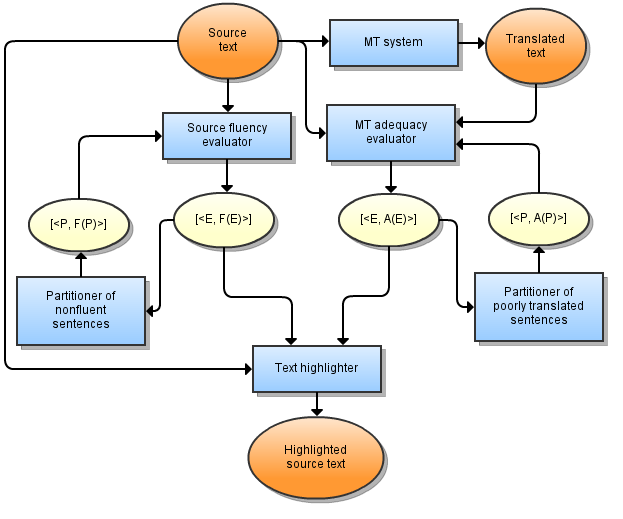
\includegraphics[width=\textwidth]{mt.png}
        \caption{Highlighting source text according to its fluency and MT quality estimation. $E$ represents a subexpression (sentence or subphrase) of the source text,
      $F$ is its fluency score, $A$ is its translation adequacy score, and $P$ is a segment of a partitioned sentence.}\label{fig:alg}
    \end{figure}
    
    The source fluency and translation adequacy highlightings are independent and can be evaluated in parallel.
    
    \subsubsection{MT adequacy highlighting}\label{sec:algad}
    The highlighting of MT adequacy is performed in the following way.
    \begin{enumerate}[(1)]
        \item\label{item:qual} 
            Given a source text that consists of $n$ sentences $S_i$, 
            evaluate the adequacy $A(S_i)$ of the translation $T_i$
            for each $i=1,\,\dots,\,n$ according to EAWR%
            ~\cite{mehdad2012match}.
            Depending on the adequacy, assign to each sentence $S_i$ a quality score
            \[
                Q_i=
                    \begin{cases}
                      3,&\text{if }A(S_i)\leq0.5;\\
                      2,&\text{if }0.5<A(S_i)\leq0.85;\\
                      1&\text{otherwise.}
                    \end{cases}
            \]
        \item\label{item:part} 
            Partition those $S_i$ for which $Q_i>1$ into $m_i$ segments $P_i^j,\ j=1,\,\dots,\,m_i$ according to~\cite{marcu1997rhetorical},.
        \item\label{item:qualpart} 
            Assign adequacy scores $Q_i^j$ to each $P_i^j$ as described in~\ref{sec:segment}, analogously to (\ref{item:qual}).
        \item\label{item:high} 
            Highlight source text in the following way:
            \begin{enumerate}[(i)]
                \item If $Q_i=2$, increase font size of sentence $S_i$ by one unit, if $Q_i=3$, increase it by two units.
                \item If $Q_i^j=2$, mark segment $P_i^j$ with a yellow background, if $Q_i^j=3$, mark it with a red background.
            \end{enumerate}
        \item Perform phrase matching as described in section~\ref{sec:concr} and remove all highlighting from the phrases that have matchings with the translated text.
    \end{enumerate}
    
    
    \subsubsection{Source text fluency highlighting}\label{sec:algflu}
    The source text fluency should only be highlighted in the worst case, when $Q=3$, for two reasons. First, because
    given that the user is fluent in the language she writes in, nonfluent text should be relatively rare.
    Second, the priority of the highlighting should be given to the MT adequacy evaluation system. Also, the user should
    not be overloaded with highlighting information that she needs to interpret.
    \begin{enumerate}[(1)]
        \item The first steps of the algorithm are analogous to steps \ref{item:qual}--\ref{item:qualpart} of~\ref{sec:algad}, 
            but instead of the adequacy evaluation function $A$ we use the source language fluency evaluation 
            $F$ based on the language model introduced in~\cite{paulslarge}.
        \item Highlighting is performed as follows:
            \begin{enumerate}[(i)]
                \item If $Q_i=3$, emphasize $S_i$ in bold.
                \item If $Q_i^j=3$, emphasize $P_i^j$ in bold and italic.
            \end{enumerate}
    \end{enumerate}
    
    
    %now: perturbation to determine which parts cause poor translation?
    

    \section{Discussion and Future Work}\label{sec:discuss}
    There are challenges and open questions to the implementation and usage of our system that need to be considered:
    \begin{enumerate}
        \item \textit{Lack of translation problem information.} Will the user understand what caused her text's translation problem when she can only see that something's wrong, rather than concrete
            information about the translation problem? Will the user have to guess how to paraphrase expressions until the translation quality likelihood
            increases? Will the bare statement of a translation problem with lack of explanation irritate the user?
        \item \textit{Excessive highlighting.} On the other hand, are three different types of text highlighting too burdensome for the user? Given that paraphrasing
            of the source text will most likely be an attempt to simplify the text or to make it more understandable, the user does not really
            benefit from knowing whether a translation quality problem emerged due to his sentence's nonfluency or ambiguity.
        \item \textit{Little fluency evaluation.} Is it really enough to focus on adequacy evaluation? Can a completely nonfluent text be adequate? 
    \end{enumerate}
        
    Additionally, the following could be done for future development:
    \begin{enumerate}
        \item \textit{EAWR on word-level.} To provide the user with more precise information on the source of the translation problem, the EAWR algorithm could
            be enhanced to the word and phrase level. This would also eliminate the necessity to run EAWR twice, on whole and segmented sentences.
        \item \textit{Paraphrasing hints.} The system could try to be more specific and give the user general hints on the improvement of a phrase. 
            For instance, it could analyze the amount of punctuation,
            number and length of segments created with the method described in~\ref{sec:segment} or the depth of possible parse trees, and tell the user
            that a sentence is too long or complicated. Another approach could be to analyze common situations that result in translation errors (see~\cite{xiong2010error})
            and give paraphrasing advice to the user if her sentence has been detected to be problematic in the terms of that model.
        \item \textit{Ambiguity detection.} The system could include detection of lexical ambiguities which are presented to the user in the same way
            as in IMT disambiguator systems. Lexical disambiguators can be automatically created using dictionaries. An open question is 
            whether the same is possible for syntactic disambiguators.
    \end{enumerate}

    
    \section{Conclusion}\label{sec:concl}
    In this paper we proposed an extension for MT systems that can help target language inexperts to improve their text's translation quality
    by highlighting the source text according to (1)~automatic translation adequacy estimation using cross-lingual textual entailment,
    and (2)~automatic source text fluency evaluation.
    
    The advantage of our approach comparing to IMT disambiguator systems is the relative simplicity of the implementation and user interface;
    we do not require to build source and target language ambiguity models, and the user does not need to be knowledgeable in linguistics
    or NLP.
    
    %\twocolumn
    \nocite{*}
    \addtocontents{toc}{\protect\vspace{\beforebibskip}}
%    \addcontentsline{toc}{section}{\refname}    
%    \bibliographystyle{plain}
    \bibliographystyle{authordate1}
    \bibliography{bibliography}
\end{document}
